\documentclass[12pt]{article}
\usepackage{url}
\usepackage[a4paper, total={6in, 8in}]{geometry}
\usepackage{hyperref}
\usepackage{titlesec}
\usepackage{graphicx}
\usepackage{amsmath}
\usepackage{amssymb}
\usepackage{mathtools}
\setcounter{secnumdepth}{4}
\usepackage{booktabs}
\usepackage{fancyhdr,graphicx,amsmath,amssymb}
\usepackage{algorithm,algpseudocode}
\usepackage{amsfonts}
\renewcommand{\algorithmicrequire}{\textbf{Input:}}
\renewcommand{\algorithmicensure}{\textbf{Output:}}

\include{pythonlisting}

\titleformat{\paragraph}
{\normalfont\normalsize\bfseries}{\theparagraph}{1em}{}
\titlespacing*{\paragraph}
{0pt}{3.25ex plus 1ex minus .2ex}{1.5ex plus .2ex}

\begin{document}

\title{WikiGaze: Wikipedia Analyzes through Gaze Based Personalized Summaries}
\maketitle

\begin{abstract}
  Due to it's complex collaborative structure and huge success, Wikipedia has been vastly analyzed from various perspectives. 
As a result, now we decently understand the overall nature of Wikipedia editors' collaboration dynamics and various features of it's articles. 
But a little research has been performed to understand readers' perspective of Wikipedia. 
In this paper, we propose a novel approach to analyze how a reader refers Wikipedia articles. 
This is attained by capturing the reading pattern of readers. 
We implement a state-of-the-art method to generate personalized summaries of Wikipedia articles through eye gaze tracking of a reader. 
These summaries capture reader's attention pattern. 
Summaries thus generated are gathered and analyzed for evaluation of different features of Wikipedia from readers' perspective. 
Using the proposed method, we develop a cross-platform document summarization and analysis tool. 
The experimental results show the efficiency of our personalized summary generation approach and the proposed analysis method of Wikipedia articles also show some interesting results.
\end{abstract}


\section{Introduction}
Wikipedia grows constantly as new entries are being continuously added by users throughout the world. This open-content encyclopedia is a unique and aptly named reference resource. It allows for public authorship and editing of any of its articles. Post inception in 2001, Wikipedia has seen exponential growth. Currently, it posses more than 48 million pages and 37 million contributors in the English Wikipedia alone~\cite{wiki:Wikipedia:Statistics}. It has been consistently ranked in the top ten visited sites on the Internet as per Alexa.com. Past studies show that Wikipedia's content quality is comparable to traditional encyclopedias~\cite{giles2005internet}. Search engines such as Google and Bing respond to user queries by extracting structured knowledge from Wikipedia~\cite{bergstrom2009conversation}.


The users of Wikipedia can be divided into two sets; the production team members(editors, moderators) and the passive team members(readers). Most of the researches performed to analyze various characteristics of Wikipedia revolve around understanding the behavior of the production teams, i.e. editors, moderators and their collaboration dynamics. A study~\cite{okoli2012people} performed on 477 Wikipedia based researches revealed that 42\% of these reseachers were centered on understanding characteristics of contributors involment or article quality evaluation~\cite{wilkinson2007assessing, kittur2008harnessing, stvilia2008information}. Only 20\% of the studies related to readers in Wikipedia and the usage of Wikipedia. Less than 1\% of the reviewed studies looked at users' reading preferences.
%and only one study investigated reading behavior~\cite{okoli2012people}. 
%performed by Okoli et al.
PageView is the technique used by Wikipedia to measure the popularity of a page among readers. It allows one to see how many people have visited an article during a given time period. This technique have several disadvantages. The statistics do not consider how long people have stayed at the article. Whether they load the article and read from begin to end, or if they leave it in seconds, it will count as one view.
In some rare cases the pageviews might have been purposely manipulated by the use of scripts or malware. Detection of such manipulations can vary in difficulty depending on the methods used.

The study by Antin et al.~\cite{antin2010readers} claims that reading can be seen as a form of participation and is therefore valuable. Reading a Wikipedia article can be considered as a legitimate peripheral participation through which individuals gain knowledge and can move towards more active participation. The fact that a user is reading an article and not editing could be interpreted as an indication of an article's quality, such as its reliability~\cite{adler2008assigning}. Thus, focus on reading activity can provide valuable insights to the article evaluation. Lehmann et al.~\cite{lehmann2014reader} emphasized on the importance of reading behavior analyses. The research characterizes users' reading preferences at article level i.e. it determines which articles are more ``engaging" than others. 

In order to perform detailed analyzes like, evaluation of a reader's attention span distribution over an article or understanding the readability issues within an article; we need to capture a reader's perception of the article. By tracking the reader's interest pattern over an article a granular analyzes can be performed. In past studies~\cite{calder2002reading, bff9c00ddce3404ca729f4a96d53a701}, it was revealed that our eye gaze pattern is closely related to our thought process. Through eye gaze tracking, we can get the knowledge about the portions of an article where a user is more focused while reading. There is evidence in research from reading psychology that eye movement patterns while reading are indeed related to textual features~\cite{rayner1978eye}.


To analyze Wikipedia articles on content level, we need a dataset containing gaze information of several users who have read a particular article. Generating such dataset requires a technique which is easy to use and available at users' site. 


\subsection{Our Contribution}

While a reader is reading a Wikipedia article, we track his eye gaze pattern using a simple \emph{web camera} and some basic computer vision techniques. Then we prepare a time-lined heatmap of the gaze intensity across the article. 

The heatmap thus produced contains a huge amount of information about the reader's reading characteristic and preferences. Its also contains some informations about the features of the article read. But utilizing a single summary we can not derive concrete results about the features of the article. Therefore we require the readers to share their gaze data for article analysis purpose.

Some readers might not be interested to share their gaze information. Therefore to incentivize readers, we automatically generate a personalized summary for the readers. The summary is personalized for the reader because we generate this summary utilising the reader's gaze information and the screen content.

The time-lined gaze heatmap indicates the areas of the article under focus. Utilizing the heatmap we extract the portions of the article where reader was more focused while reading and generate a summary for him. Reader is also allowed to provide his requirement for the length of the summary. According to the length requirement we decide the threshold to perform text extraction from the article. 

Peter et al.\cite{dunn2019evaluating}, mentions that the the role and purpose of Wikipedia is not to act primarily as a comprehensive learning resource but more as a quick reference tool. In researches like \cite{olsen2012just, head2010today}, it has been found that Wikipedia articles are not read from start to end. Instead most of the readers refer these articles to enhance their knowledge over a particular context of the topic. In \cite{head2010today} it is also mentioned that readers use Wikipedia to summarize their knowledge over a topic. Therefore it will be highly beneficial, if we facilitate readers to automatically prepare summary of an article as they read it.

%%%%%%%%%%%%%%%%%%%%%
%\cite{head2010today} How today's college students use Wikipedia for course-related research\\
%How frequently college students use Wikipedia.\\
%What motivates students to use Wikipedia.------> Summary\\
%At which stages of research students use Wikipedia.\\
%How Wikipedia is used in relation to other information resources.\\
%What predictors reveal which types of students are more and less likely to use Wikipedia.\\

%Mention that Wiki is mostly referred and not read from top to bottom. It will be highly useful if we can create summary of articles.
%Store off-line so that in absence of Internet we can access the content. Update the summary as per updated requirement.

%\cite{dunn2019evaluating}
%the role and purpose of Wikipedia is not to act primarily
%as a comprehensive learning resource but more as a quick reference tool.
 
%We ask the users to share their gaze information for analyzes purpose.  Due to privacy reasons, some users might not be willing to share their data. As an incentive mechanism we facilitate users to generate a personalized summary for the article which they read. The personalized summary is automatically generated utilizing reader's gaze information and screen content.
%%%%%%%%%%%%%%%%%%%%%

We develop a cross-platform standalone application to generate personalized summaries for Wikipedia readers. This application automates the tasks of summary creation and \textbf{uploads the summary on a centralized server} for further analysis purpose. For a particular article, we gather all the summaries uploaded and utilize them for the article analysis purpose. 

%%%%%
%Recommendation system: article title and generated summary
%%%%%%

%%%%%%%
%PageView is the current technique to see if users have visited any web page but it has several disadvantages like.....\\
%\cite{wiki:Wikipedia:Pageview_statistics}\\
%The statistics do not consider how long people have stayed at the article. Whether they load the article and read from begin to end, or if they leave it in seconds, it will count as one view.
%In some rare cases the pageviews might have been purposely manipulated by the use of scripts or malware. Detection of such manipulations can vary in difficulty depending on the methods used.
%Give page view formula
%%%%%%%
The summary dataset reflects readers intake of various articles. To the best of our knowledge no such datset exists. On this dataset various analyzes results can be produced. In this paper we show two such analyzes. The first analyzes prepares a leader-board for Wikipedia editors based on their content contribution presence in various summaries. This leader-board is prepared on article level. The rational behind this analyzes is to judge editors' contribution based on the extent to which it is being read by other users. In second analyzes we try to find the correlation between summary length and article length. This is to analyze if users get discouraged by long article and read less or the length of an article does not effect the reading extent. We discuss analyzes results in later sections.  

The key contribution of our work is as follows:
\begin{itemize}
	\item A state-of-the-art approach to generate personalized summaries based on eye gaze tracking.
	\item A novel approach to analyze Wikipedia articles based on users' reading pattern.
	\item Development of a cross-platform application to generate personalized summaries and recommend summaries.	
\end{itemize}


\subsection{Paper Structure}
The structure of rest of the paper is as follows. \hyperref[sec:Related]{Section 2} points on some of the related works. \hyperref[sec:Proposed]{Section 3} explains the proposed analyzes technique for Wikipedia. In \hyperref[sec:Analysis]{Section 4} we explain how the proposed technique can be utilized to analyze Wikipedia articles. \hyperref[sec:Resources]{Section 5} explains the online resources provided. \hyperref[sec:Discussion]{Section 6} contains a detailed discussion on the proposed method. \hyperref[sec:Conclusion]{Section 7} concludes and discusses future work.


\section{Background \& Related Work}\label{sec:Related}
Wikipedia research community can be vastly divided into two classes: one that \emph{uses} Wikipedia as a source of knowledge and other that \emph{studies} Wikipedia. Our research falls in both the categories. We \emph{use} Wikipedia to \emph{study} Wikipedia. We generate a dataset containing summaries of Wikipedia articles and also utilize this dataset to analyze the articles.

In this section we describe the theoretical background and related previous works in the fields of automatic document summarization and various methods of Wikipedia analysis. First, we review user awareness in utilization of eye gaze data for determining reader's interest and thus generation of personalized summary. Then, we also review the literature on Wikipedia analysis methods.

\subsection{Relation between Eye Gaze and Readers Interest}
Eye movement characteristic of reading is extensively studied in the psychology literature~\cite{rayner1998eye}. Eye tracking open the door for an automated analysis of document reading. The time-lined distribution of saccades and fixations reflects significant features of the reader as well as the text being read. In a study performed by Frazier at al. \cite{frazier1982making} regressions indicate the disambiguation of a sentence. In addition long regressive eye movements (regressing more than 10 letter spaces~\cite{rayner1998eye}) may indicate difficulty in understanding the text (\cite{frazier1982making} \cite{rayner2012eye}. 

The relation between eye gaze pattern and human interest has been vastly utilized in various fields~\cite{knight2013estimating}. In~\cite{beymer2005webgazeanalyzer} a system is proposed for recording and analyzing web reading behavior using eye gaze. In \cite{bee2008writing}, a gaze-controlled input system was introduced that enables users to write with their eyes. Sanches et. al~\cite{sanches2018estimation} show that prediction of the subjective understanding is improved by 13\% if we use eye gaze instead of comprehension questions. Eye gaze is also used for website designing~\cite{djamasbi2014eye}. 

Considering all the instances discussed above, we can say that eye gaze reflects the interest of the reader. Therefore it can be used to segregate the portions of the document where reader was interested while reading from the portions that he skimmed through or did not read at all.


\subsection{Personalized Summarization Techniques}
%title = Single Document Summarization as Tree Induction

Summarization is the task of automatically generating a shorter version of a document while retaining its most important information. The task has received much attention in the
natural language processing community due to its
potential for various information access applications. Examples include tools which digest textual
content (e.g., news, social media, reviews), answer
questions, or provide recommendations.
Of the many summarization paradigms that
have been identified over the years (see \cite{autoSum}
and {Nenkova, Ani, and Kathleen McKeown. "Automatic summarization." Foundations and Trends$^{\tiny{\textregistered}}$ in Information Retrieval 5.2–3 (2011): 103-233.}
for comprehensive overviews), two have consistently attracted
attention. In abstractive summarization, various
text rewriting operations generate summaries using words or phrases that were not in the original
text, while extractive approaches form summaries
by copying and concatenating the most important
spans (usually sentences) in a document. 

%title = Neural Latent Extractive Document Summarization

A great deal of previous work has focused
on extractive summarization which is usually modeled as a sentence ranking or binary classification problem (i.e., sentences
which are top ranked or predicted as True
are selected as summaries). Early attempts
mostly leverage human-engineered features
(Filatova and Hatzivassiloglou, 2004) coupled
with binary classifiers (Kupiec et al., 1995), hidden Markov models (Conroy and O’leary, 2001), graph based methods (Mihalcea, 2005), and integer linear programming (Woodsend and Lapata,
2010). Although seemingly more successful than their
abstractive counterparts, extractive models require
sentence-level labels, which are not included in
most summarization datasets (only document and
gold summary pairs are available). Sentence labels are usually obtained by rule-based methods (Cheng and Lapata, 2016) or by maximizing
the ROUGE score (Lin, 2004) between a subset
of sentences and the human written summaries
(Nallapati et al., 2017). These methods do not
fully exploit the human summaries, they only create True/False labels which might be suboptimal.




Personalized summarization... personalization in different contexts like review summarization {Towards Personalized Review Summarization via User-Aware Sequence Network}, chat summarization {Collabot: Personalized Group Chat Summarization}, personalized web graph visualization {UIWGViz: An architecture of user interest-based web graph visualization}, personalized web search {Summarizing local context to personalize global web search}
, personalized tweet summarization {Personalized time-aware tweets summarization}, {Personalized and automatic social summarization of events in video}


personalized document summarization:
1.) WebInEssence: A Personalized Web-Based Multi-Document
Summarization and Recommendation System
2.) Personalized PageRank Based Multi-document Summarization
3.) Automatic query-based personalized summarization that uses pseudo relevance feedback with NMF
4.) Personalized Document Summarization Using Non-negative Semantic Feature and Non-negative Semantic Variable
5.) Personalized text summarization based on important terms identification
6.) Summarize what you are interested in: An optimization framework for interactive personalized summarization


Current information retrieval (IR) systems rely mostly on explicit, typed queries,
combined with explicit feedback telling the system which of the search results were
relevant. The relevance feedback is used to refine the query, and the search converges
iteratively towards more relevant documents.


Eye gaze based summarization...
   



\subsection{Wikipedia Analysis Techniques}
\cite{chevalier2010wikipediaviz} There have also been quantitative studies that attempt to assess the
quality of Wikipedia articles in a more objective way using metrics based on the meta-data associated with Wikipedia itself. Blumenstock simply uses the word count of an article as a measure of
quality~\cite{blumenstock2008size}. Lih  has suggested the number of edits and unique
contributors of an article as measure for quality, where the number
of unique authors reveals the diversity of an article and the number of edits its rigor. Wilkinson et al. have demonstrated later
that high-quality vs. non-featured articles have indeed substantially
more contributors involved [25]. In [1], these two measures are
combined to define the notion of author reputation. Other single metrics based on the aggregation of several indicators have been
proposed to predict the quality of a contribution [7] or the trustworthiness of an article [6]. In addition the collaborative work in
dedicated discussion pages — where changes are often discussed
before being introduced in the article [21] — plays a critical role in
the quality of articles [11, 23].
A common trend in these studies is that the metrics reveal social
information that can be used as an indicator for assessing the quality of an article. It has been shown that revealing trust-relevant
information to the users has an effect on the trustworthiness of the
articles [12, 15], and three visual tools have been proposed aiming
at enhancing the user and reader experience on Wikipedia.



\section{Methodology}\label{sec:Proposed}

Cross-platform application (Ubuntu, Mac, Windows)...Application detail...\\
1: Summarization (basic feature...)\\
2: Summary recommendation (advanced feature...)


We present a novel approach to analyze Wikipedia articles by capturing the reading pattern of users, through personalized summaries. 

\subsection{Personalized Summarization}

Document summarization reflects the key points of the document which the summarizer tool deems important. The summary thus produced is generic in nature. In many situations, users are interested in facts more relevant to them; motivating the need for query-relevant or personalized summaries. For instance, consider a sports enthusiast who wants to know about the sports culture in United States by reading its' Wikipedia article. A more useful summary for this person would contain sports related passages assembled into a short document. We can say that users with different information needs require different summaries of the same document.

Personalization has been identified as being one of the grand challenges in information retrieval lately~\cite{belkin2008some}. Personalized summarization~\cite{berkovsky2008aspect} presents users with document extracts that are of interest to them. Manual filtering of information from large documents is a tiresome task. Therefore it becomes extremely significant to automate this process. Majority of the automatic personalized summarization techniques incorporate some kind of personal information for individually improving the quality of summary~\cite{moro2012personalized, wu2008personalized, kumar2008generating}. The proposed technique does not require the users to share any personal information. 

%%%%%%%
Include similar sections of the article as per our selected portions.
%%%%%%%


Spacial and temporal gaze patterns are valuable pieces of information and can be used to infer present cognitive processes of the user \cite{Beymer:2005:WSC:1056808.1057055}. We utilize the eye gaze pattern to extract more focused portions of the text and assemble them to generate personalized summary. In following subsections, we address methods and measures to generate a summary.

\subsubsection{Eye Gaze Tracking}
Eye gaze tracking is the process to estimate the direction of gaze and the point of regard. Rayner~\cite{rayner1998eye} provides a comprehensive overview of the studies concerning gaze pattern while reading. The eye shows a characteristic behavior composed of a series of fixations and saccades. Fixation is a duration for which the eye is steadily gazing at one point. On average it is of time interval 200-250 ms. Saccade is a rapid eye movement from one fixation to the next. For languages written left-to-right; approximately 10-15\% of the eye movements during reading are regressions, i.e., movements to the left along the currently focused line. A regression, or backwards eye movement in the text, is a sign that the
reader is having difficulty understanding the material.

Well established devices, like Tobii~\cite{olsen2012tobii}, EyeLink~\cite{cornelissen2002eyelink}, etc. are available for gaze tracking. Though they provide higher accuracy, they are quite expensive and rarely available at user's site. Applying eye tracking to reading analysis requires a basic trade off between the invasiveness of the eye tracker and the accuracy of the estimated gaze points. To collect the dataset of Wikipedia reader's gaze pattern, we require a feasible, easy to use solution. 
Therefore we obtain gaze samples through vision-based commodity eye tracking. We assemble an eye-tracking setup containing a Logitech Webcam C922 Pro Stream and readily available eye-tracker applications. Table 1 shows the details of the eye-trackers used for various platforms. 
The main reason behind selecting these trackers is to make our tool platform independent. CVC ET~\cite{ferhat2014cheap, CVC} is the port of Opengazer for the Linux and Mac platform and NetGazer~\cite{WinNT} is the port of Opengazer for the Windows platform. CVC ET as well as NetGazer are open-source softwares. The CVC ET is actively maintained by researchers from Universitat Aut\'{o}noma de Barcelona~\cite{CVC}. It provides 1.47$^{\circ}$ horizontal error and 1.35$^{\circ}$ vertical error. NetGazer is not maintained anymore therefore we updated the package based on CVC ET functions; since they both are based on Opengazer project. 

\begin{table}[]
\begin{tabular}{|c|c|c|c|c|c|c|}
\hline
Tool     & Language & Platform  & Vertical Error & Horizontal Error & License & Reference                     \\ \hline
NetGazer & C++/C\#  & Windows   & 1.55$^{\circ}$ & 1.62$^{\circ}$   & GPLv2   & \cite{WinNT} \\ \hline
CVC ET   & C/C++    & Linux/Mac & 1.35$^{\circ}$ & 1.47$^{\circ}$   & GPLv2   & \cite{CVC}   \\ \hline
\end{tabular}
\caption{Detail of eye-trackers used for various platforms.}
\label{tab:eye_tracker}
\end{table}

To meet our requirement we modified some of the functions of the eye-trackers. The assembled setup containing a simple camera and the selected eye-trackers, is non-invasive, cost effective and platform independent. 


Using Webcam, we record reader's facial video and feed this as input to the eye-tracker. Eye tracker detects eye gaze direction in the video and maps the gaze to the location on the screen where the user is looking at. 


Mathematical formula for gaze mapping on screen...

This process continues during the entire reading session. The time-series data of on-screen gaze locations are captured. 



\subsubsection{Frame Recording \& Wikipedia Specific Text Extraction}

Ajanki et.al~\cite{bff9c00ddce3404ca729f4a96d53a701} claim that when the system has no prior information as to what the user is searching, the eye movements help significantly in the search. This is the case in a proactive search, for instance, where the system monitors the reading behaviour of the user in a new document. Xu et al.~\cite{xu2009user} talk about the relevance between the human text reading pattern and their current cognitive process. Their basic assumption is that the eyes' fixation duration on a word is directly equivalent to the user's interest in that word. 


%%CHANGE%%
First, our reading analysis deals
with inherent noise and drift problems in remote trackers –
fixations are grouped along horizontal scans and matched
against the text DOM lines in a robust manner. While
mapping a single fixation to the text lines may be
ambiguous, the matching of groups of fixations to chunks
of the DOM can resolve this ambiguity. 
%%CHANGE%%

Based on these assumptions we create a sentence ranking mechanism based on the duration for which it was being gazed by a user.

equation to identify the "selected area" for text extraction.

\cite{c7691a9428684758a206610e6bd9ee3e} paragraph based text extraction.

Generate heat map using:
Identify the thresholded contours on the image:
Extract the text from image:

Based on heat-map we extract text from images. Bounding box formation : wiki specific


To optimize the summarization process, we are do not record the entire article reading video; instead we only store the required frames. We identify the frames by considering the human reading pattern. According to the study performed by Rayner et al. \cite{rayner2010eye}, the average reading speed for fast readers is about 330 wpm (words per minute) and that for slow readers is about 200 wpm. Sichel \cite{sichel1974distribution} performed a number of experiments and showed that most of the sentences contain 11-15 words. The text extraction is done on sentence level. To decide on the frame recording we need to consider the boundary condition which is of fast reader (330wpm) and less number of words(11). This results in 2 seconds time to wait before frame recording. Therefore, we are recording frame after every 2 seconds of frame change event. As long user is reading text on the same screen we are not saving the frame.

        
        
\subsubsection{Summarization}
%We have implemented two layers of summarization..


The main goal of extractive summarization can be
concisely formulated as extracting from the input
pieces of text which contain the information about
the most important concepts mentioned in the input
text or texts. This definition conceals a lot of important issues that should be taken into consideration
in the process of summary construction

what does it depict?


%\paragraph{Abstractive Summarization}
%abstractive summarization systems generate new phrases, possibly rephrasing or using words that were not in the original text


%\subsection{Summary Recommendation System}
%%%%%%%%change%%%%%%%%
%    One possibility is that having many
%contributors results in higher quality and less biased articles.
%The benefits of aggregating judgments from many people
%have been observed since at least 1907, when Galton showed
%that averaging independent judgments of many observers
%estimated the weight of an ox at a county fair better than
%experts could [7]. The Internet makes aggregating
%judgments much easier, leading to systems of collective
%intelligence ranging from markets for accurately predicting
%presidential elections [3] to systems where volunteers
%classify craters on Mars' surface, resulting in work virtually
%indistinguishable from that of expert geologists [17]. Most
%models of collective intelligence are premised on
%aggregating the independent contributions of many people,
%colloquially known as harnessing ``the wisdom of crowds" [32]
%%%%%%%%change%%%%%%%%
%
%
%Paper on recommending personalized summary \cite{cagliero2019recommending}


\section{Wikipedia Analysis}\label{sec:Analysis}
Based on the summary created, we can capture the article reading pattern. This can serve as a novel dimension to analyze Wikipedia articles. 

    
\subsection{Editor's Contribution Analysis}
Wikipedia is a crowd-sourced online community for knowledge building. A characteristic feature of such online communities and social media sites is the mechanism for rewarding user achievements. It is primarily done to motivate users to enhance their on-site participation. There exists a strong correlation between editor contribute and article quality~\cite{li2015automatically}. 
Leaderboards are commonly used by participants to compare their performance against others and reward them by publically enhancing their rank. Blum et. al~\cite{blum2015ladder} show the importance of leaderboard creation and how participants' ranking affects their future performance.

Each editor in Wikipedia contributes some facts to the article. Therefore a naive way to rank editors' contribution is by comparing their individual contributions in bytes. This method has several prominent disadvantages, like the quality of the contribution will not be captured this way. An editor who adds much random text in the article can be ranked higher than an editor who contributes 2-3 relevant sentences. There have been several attempts to understand the collaboration dynamics of Wikipedia editors~\cite{kim2016understanding, sepehri2012leveraging, wagner2016women}. These studies evaluate the performance of production side users, like, editors from the article content production perspective alone. 

In the proposed evaluation technique we bring in the perspective of passive side users, i.e., readers. This will enable capturing the perception of editors content contribution by it's readers. An editor who's contribution is more referred by readers can be assumed to have a better understanding of the readers requirement and therefore should be given higher preference in leaderboard. Using the personalized summaries gathered for an article, we create a model to rank it's editors contribution. 

Given a personalized summary, we create a list of all the editors whose content appear in this summary. This list is created by tracing back along the article revision history to search which editor first added that particular content. 

\textbf{Formula to rank editors}\\
How much?\\
How old?\\
In how many?\\

$R$ is the list of all the valid revisions i.e. excluding vandals and where number of bytes modified is greater then 10.

$E$ is the list of authors who contributed for valid revisions.
$\forall i \in (0, N)$ where $N$ is the number of valid revisions; $e_i \in E$ implies $e_i$ is the editor of $i^{th}$ revision.



$E$ is a nested dictionary containing unique list of editors of an article with different ranks for each summary. The first level contains a pointer to the dictionary of editors for each summary. The second level contains a dictionary for each editor of the article under consideration with their contribution score initialized to zero.
%$E$ is formed keeping in consederation the time when an edits makes his/her first edit. This is done to keep into account the logitivity of their text.
Let $S$ be the set of summaries based on which the article is evaluated.


\begin{algorithm}[H] 
\caption{Similarity Score Calculation}
\label{alg:sim_score}
\begin{algorithmic}[1]
\Require{$r_i$, $s_j$}
\Ensure{Similarity score for an editor based on his/her contribution in S} 
\Statex
\Function{SimilarityScore}{$r_i$, $s_j$} %{$A[\;]$}
	\State{$s\_{sent}$ $\gets$ list of senetences in $s_j$}
	\State{$r\_{sent}$ $\gets$ list of senetences in $r_i$}
	\State $total\_score$ $\gets$ $0$
	\For{$k \gets 0$ to len($s\_{sent}$)}	
		\State {$match \gets$ ``best match" of $s\_{sent}[k]$ in $r_i$}
		\State {$s\_vec \gets$ vectorize($s\_{sent}[k]$)}
		\State {$match\_vec \gets$ vectorize($match$)}		
		\State {$score \gets$ cosine($s\_vec$, $match\_vec$)}
		\State {$total\_score \gets total\_score + score$}
    \EndFor
    \State \Return {$total\_score$}	
\EndFunction
\end{algorithmic}
\end{algorithm}


\begin{algorithm}[H] 
\caption{Editors Leaderboard Creation}
\label{alg:Leaderboard}
\begin{algorithmic}[1]
\Require{$R$, $S$, $E$} 
\Ensure{Sorted list of editors based on their content in S} 
\Statex
\Function{Leaderboard}{$R$, $S$, $E$}
	\For{$s_j$ in $S$}     
		\State {$score\_old \gets 0$}\Comment{$E_j$ is the list of editors for summary $s_j$}
        \For{$r_i$ in $R$}\Comment{$e_a \in E_j$ is the editor for revision $r_i$}
        	\State {$score \gets$ SimilarityScore($r_i$, $s_j$)}
        	\If {$score\_old$ == $score$}
        		\State {$editor\_score \gets 0$}
         	\Else
        		\State {$editor\_score \gets score - score\_old$}
        		\State {$score\_old \gets score$}
        	\EndIf
        	\State $e_a \gets e_a + \frac{1}{i} * editor\_score$ 
        \EndFor
    \State {$E_j \gets$ Sort($E_j$)}
    \EndFor
    \State {Update $E_j$ in $E$}
    \State \Return {$E$}
\EndFunction
\end{algorithmic}
\end{algorithm}


The ``best match" is found by using ``get\_close\_matches" function of ``difflib" package with a cutoff of 0.5.
% so that it matches only with highly similar sentences.


Editor for revision $i$ will get 0 score the matching score is same for $i^{th}$ and $(i-1)^{th}$ revision. This is because this editor has not done any contribution in the text which is present in this summary.

Editor for revision $i$ will get negative score the matching score for $i^{th}$ revision is less than the score  for the $(i-1)^{th}$ revision.  Negative score implies that the editor for revision $i$ has adversely modified the text which appeared in summary. 

Editor for revision $i$ will get positive score the matching score for $i^{th}$ revision is greater than the score  for the $(i-1)^{th}$ revision. Positive score implies that the editor for revision $i$ has constructively modified the text which appeared in summary. 


In \ref{alg:Leaderboard}, line 11, we can see for editor ($e_i$) of revision $r_i$ we calculate the editor score using following formula:
$$e_a \gets e_a + \frac{1}{i} * editor\_score$$

Weighted sum of the score of an editor accross all the revisions. We use inverse of revision index as weighting factor to take into consederation the longitivity of the contribution. There can be a situation that an editor's edits are modified but they must be coming back in the article because they are finally appearing in the current revision.

Vectorize() explain...

We sort this list as per editor's contribution bytes present in the summary and rank the editors. Editors rank is zero if his contribution is not present in a summary. For all the summaries of a particular article this process is repeated. Each editor is given a score which is a function of editors rank in a summary and the number of bytes of his contribution content in the summary.   



\begin{figure}[!htb]
        \center{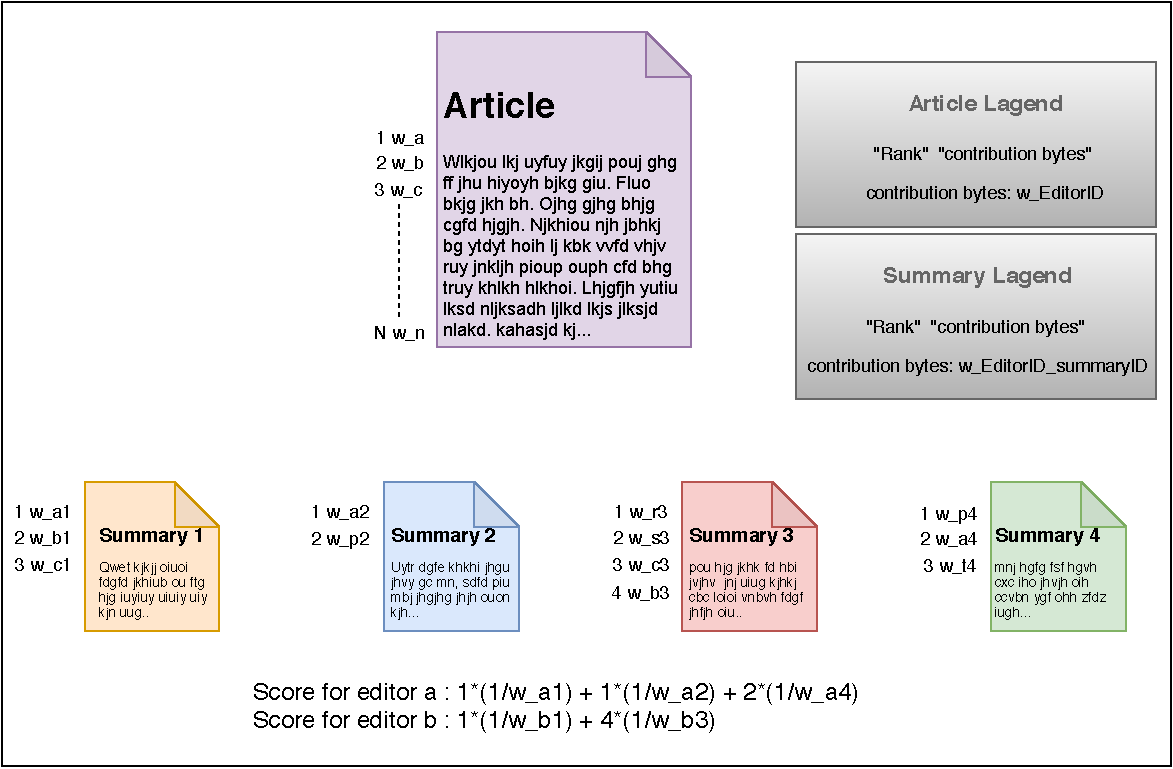
\includegraphics[width=15cm]
        {images/editor_contrib.pdf}}
        \caption{\label{fig:editor_contrib} Formula to calculate editor score}
\end{figure}

General formula to calculate editor ($x$) score:

\begin{equation}
	Score_x = \sum_{k=0}^{k=m}I_x(k)\begin{bmatrix}R_x(k).\frac{1}{w\_xk}\end{bmatrix}
\end{equation}

    where, $m$ is the number of summaries of article under consideration. $I_x(k)$ is an indicator function. 
If $I_x(k)=1$, it implies that summary $k$ contains content contributed by editor $x$ and 0 otherwise.
$R_x(k)$ refers to the rank of editor $x$ in summary $k$ and $w\_xk$ refers to the number bytes present in the summary $k$ which was contributed by editor $x$.

The lower the score, the better the rank of an editor on leaderboard. The score is directly proportional to the rank of an editor in a summary and inversely proportional to the contribution bytes in that summary. This is done to nullify the impact of varying summary lengths.



Table of analyzes for editor ranking in an article and our ranking.


    
%\subsection{Relation between Summary Length \& Article Length}
%\subsection{Relation between Article Length and it's Reading Extent}    
%Article length is considered an effective metric for analysing an article~\cite{chevalier2010wikipediaviz, dang2016quality}.   Falagas et. al~\cite{falagas2013impact} demonstrates the impact of article length on the number of citations that it might get in future. Blumerstock ~\cite{blumenstock2008size} shows that article length is a critical parameter  to differentiate featured articles from other articles in Wikipedia. 
%But it can not be said that all long articles are good.~\cite{blumenstock2008size} shows several counterexamples that prevent using it alone as a quality measure.
%
%While article length plays an important role in analyzing an article from various aspects, does it actually motivate a reader to read the article more or it discourages the reader to read it completely. Readers can be considered as clients for a Wikipedia article. Therefore it becomes essential to analyze the correlation between the length of an article and the extent to which it is read by users.
%
%To determine the relationship between article length and it's reading extent
%we need a mechanism to capture how much an article is read by a user. This is facilitated by the personalized summary that we create by analyzing user's reading pattern. Summary demonstrates the portion of the article which was read with focus. Therefore, we can use the summary length to measure the reading extent of an article.
%
%
%
%plot of different summary lengths of an article (long article \& short article)
%
%plot of article length and average summary length
%
%
%
%Conclusions....

    
    
\subsection{Relation between Gaze Pattern and Article Readability}    
Automating the process of measuring the quality of a Wikipedia article has been an important task since last ...... Several attempts have been made in this regard....
cite....
cite....
cite....




%%%%%%%%%%%%%%%%%%%%%%%%%%%%%%%%%%%%%%%%%5
FRE uses both the average number of syllables per word and the average number of words per sentence to estimate the reading level.

\begin{equation}
FRE = 206.835 - 1.015\begin{pmatrix}
\frac{words}{sentence}
\end{pmatrix} - 84.6\begin{pmatrix}\frac{syllables}{word}\end{pmatrix}
\end{equation}

where `words', `sentences' and `syllables'
entail the number of each in the text, respectively.
FRE was chosen due to its popularity and consistency with other
readability metrics \cite{didegah2013factors, kincaid1975derivation}

%Here we are using a variant of Flesch Reading Ease (FRE) proposed by  Kincaid et al. \cite{kincaid1975derivation}. It calculates grade level (GL) 

Jumbled sentences((x,y) values) and FRE value correlation \textbf{plot}. 
(x,y) values should be more jumbled (plotted over a number of summaries) for higher FRE value.

Number of people have difficulty reading the article (lot of back eye movements) should correlate with the higher FRE value.


Flesch-Kincaid Grade Level

Most of the readability algorithms can produce results outside the score range, when they do not limit content size.

Give out of scorecard values if text is very small. When tried to find readability on sentence level it gave negative value. Our method works at sentence level.

Block time FKGL and block time by summing up each line's time.
Mention the meaning of different range of values of FKGL.


%
%NDC scores are calculated by using the percentage of difficult words and the average sentence length of abstracts. While the NDC was
%originally calculated on 100 words due to
%computational limitations, we used the entire
%text.
%\begin{equation}
%	NDC = \begin{Bmatrix*}[l]
%
%0.1579\begin{pmatrix}
%\frac{difficult}{words} * 100 
%\end{pmatrix} +0.0496\begin{pmatrix}\frac{words}{sentences}\end{pmatrix} + 3.6365
% & if \begin{pmatrix}
%\frac{difficult}{words}
%\end{pmatrix} >5 \\
%
%0.1579\begin{pmatrix}
%\frac{difficult}{words} * 100 
%\end{pmatrix} +0.0496\begin{pmatrix}\frac{words}{sentences}\end{pmatrix}
% & if \begin{pmatrix}
%\frac{difficult}{words}
%\end{pmatrix} \leqslant 5
%\end{Bmatrix*}
%\end{equation}
%
%
%where `words', and `sentences' entail the number of each in the text, respectively. `Difficult' is the number of words that are not present in the NDC common word list. NDC has been shown to perform comparably with these more modern methods (\cite{benjamin2012reconstructing}
%%%%%%%%%%%%%%%%%%%%%%%%%%%%%%%%%%%%%%%%5


All these approaches require devising a complex feature set or using some machine learning approach to quantify the quality of an article. 

In the proposed approach we try to find out the relationship between article quality and gaze pattern.

Samples grid...

Features of gaze heatmap to evaluate article quality...

plot for these features...

Conclusions...

\section{Experiment and Results}
In this section we evaluate the quality of our article summarization tool and we also discuss the results of various Wikipedia analyses proposed. 


\subsection{Dataset}

We collected the set of articles from the categories "Multi-year ranking of most viewed pages". We recorded and analyzed gaze data from *** participants, all being graduate or undergraduate university students 
majoring in a variety of different subjects.


\begin{figure}[!htb]
    \center 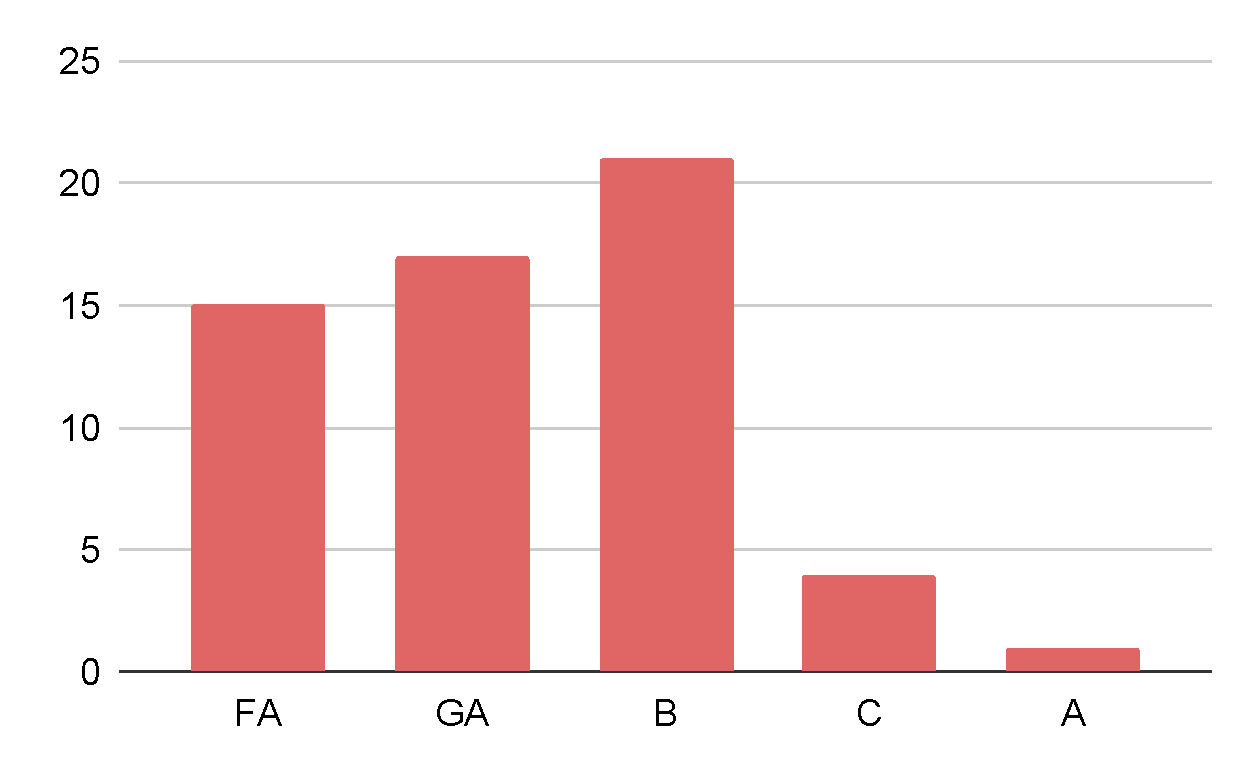
\includegraphics[width= 9cm]{images/article_category.pdf}
    \caption{\label{fig:article_category} Count articles belonging to various categories}
\end{figure}


\subsection{Summarization}
The intrinsic approach quantifies the performance of the summarization technique on the basis text coverage comparison with a ground truth summarization result. 


Avg P:0.21093474426807765\\
Avg R:0.40370370370370373\\
Avg f\_measure:0.2723123123123123\\

Recall: 0.5
Precision: 0.18518518518518517
f\_measure: 0.2702702702702703

Other tool (mentioned at https://ivypanda.com/online-text-summarizer):\\
\begin{itemize}
\item Autosummarizer: 0
\item Smmry: 0
\item Summarizing.biz: 0
\end{itemize}

\subsection{Results of Analyses}


\subsubsection{Editor's Contribution Analysis}
\cite{adler2007content} authors gain reputation when the edits and text
additions they perform to Wikipedia articles are longlived, and they lose reputation when their changes are
undone in short order. \textbf{FIND MORE IN ITS CITATION} \\
\cite{adler2008measuring} We consider and compare various alternative criteria that take into account the quality of a contribution, in addition to the quantity, and we analyze how the criteria differ in the way they rank authors according to their contributions. As an outcome of this study, we propose to adopt total edit longevity as a measure of author contribution.

 Contributors tool 
 %(https://xtools.wmflabs.org/articleinfo/en.wikipedia.org/Stephen%%20Hawking)
 Find Top 10 contributors. 

%%%%%%%%%%%%%%%%%%%%%%%%%%%%%%%%%%% change
1.2.2. Top editors
The top editors section shows various information about users and bots who have edited the page. There are two pie charts comparing the top editors by number of edits and by added text. XTools does not count bot accounts as a top editor. Instead, they are listed in the bot list table.

1.2.2.1. By number of edits
The Top 10 by edits chart compares the number of edits each top editor made. The percentages shown in parentheses refer to the number of edits the user made in relation to total number of edits made to the page.

1.2.2.2. By added text
Added text refers to any positive addition of content that was not reverted with the next edit. This is because users who fight vandalism (for instance) will otherwise appear to have added a lot of content to a page, when in actuality they just undid an edit that removed a lot of content. Going by edits that weren't reverted, we have a better idea of the users who made meaningful contributions.

Note however that the Page history tool only detects reverts if it happened with the very next edit, and not a later edit.

The “Top 10 by added text” pie chart compares each of the 10 top editors. The percentages shown in parentheses refer to the amount of content that user added compared to all content that was added to the page.

1.2.2.3. Top editors table
The first table shown lists the top editors (non-bots) and various statistics about their contributions to the page. The last two columns show specialized calculations. Average time between edits (atbe) is the average number of days between each of the user’s edits to the page. This is starting with the date of their first edit and the date of their last edit to the page. Added (bytes) refers to the number of bytes of text the user added to the page.

By default only the first 20 editors are shown. You can expand to show all editors using the link on the bottom row of the table.

You can also export this data as wikitext using the link just above the table.

1.2.2.4. Bot list
The “Bot list” shows lists all of the bots that edited the page, ranked by edit count. A message is shown indicating if the bot is no longer a bot, and links to the account’s user rights log.

The list is by default limited to the top 10 bots. You can expand to show all bots using the link on the bottom row of the table.


\begin{table}[]
\begin{tabular}{@{}cccc@{}}
\toprule
Rank & Username          & Edits & Bytes Added \\
\cmidrule(r){1-1}\cmidrule(lr){2-2}\cmidrule(l){3-3} \cmidrule(l){4-4}
1    & Slp1              & 268   & 43,304      \\ 
2    & Fayedizard        & 256   & 12,022      \\ 
3    & Drbogdan          & 94    & 13493       \\ 
4    & SandyGeorgia      & 45    & 772         \\ 
5    & Dodger67          & 43    & 436         \\ 
6    & TimothyRias       & 40    & 2285        \\ 
7    & MathewTownsend    & 39    & 2832        \\ 
8    & John              & 36    & 37          \\ 
9    & Materialscientist & 31    & 300         \\ 
10   & Nightscream       & 31    & 1491        \\ 
\bottomrule
\end{tabular}
\caption{Top 10 editors list generated by XTools for "Stephen Hawking" Wikipedia article as of 28 December 2019. }
\label{tab:Xtool_editor}
\end{table}




\begin{table}[]
\begin{tabular}{@{}ccccc@{}}
\toprule
Rank & Username          & Edits & Minor Edits \% & Bytes Added \\
\cmidrule(r){1-1}\cmidrule(lr){2-2}\cmidrule(l){3-3} \cmidrule(l){4-4} \cmidrule(l){5-5}
1    & SlimShady6135  & 438   & 3.7\%         & 67,450      \\
2    & SNUGGUMS       & 316   & 9.5\%         & 2,759       \\
3    & STATicVapor    & 288   & 7.6\%         & 15,018      \\
4    & Angelic Wraith & 244   & 59.4\%        & 31,851      \\
5    & Banan14kab     & 138   & 0\%           & 2,722       \\
6    & Udonknome      & 130   & 27.7\%        & 5,541       \\
7    & Wikien2009     & 123   & 2.4\%         & 13,091      \\
8    & Vacanzeromane  & 111   & 15.3\%        & 6,321       \\
9    & AJS2050        & 111   & 2.7\%         & 14,150      \\
10   & Arbor to SJ    & 101   & 21.8\%        & 9,602       \\ 
\bottomrule
\end{tabular}
\caption{Top 10 editors list generated by XTools for "Eminem" Wikipedia article as of 28 December 2019. }
\label{tab:Xtool_editor}
\end{table}

%%%%%%%%%%%%%%%%%%%%%%%%%%%%%%%%
 
 Use our approach to find top 10 contributors.
 
\begin{figure}[!htb]
    \center 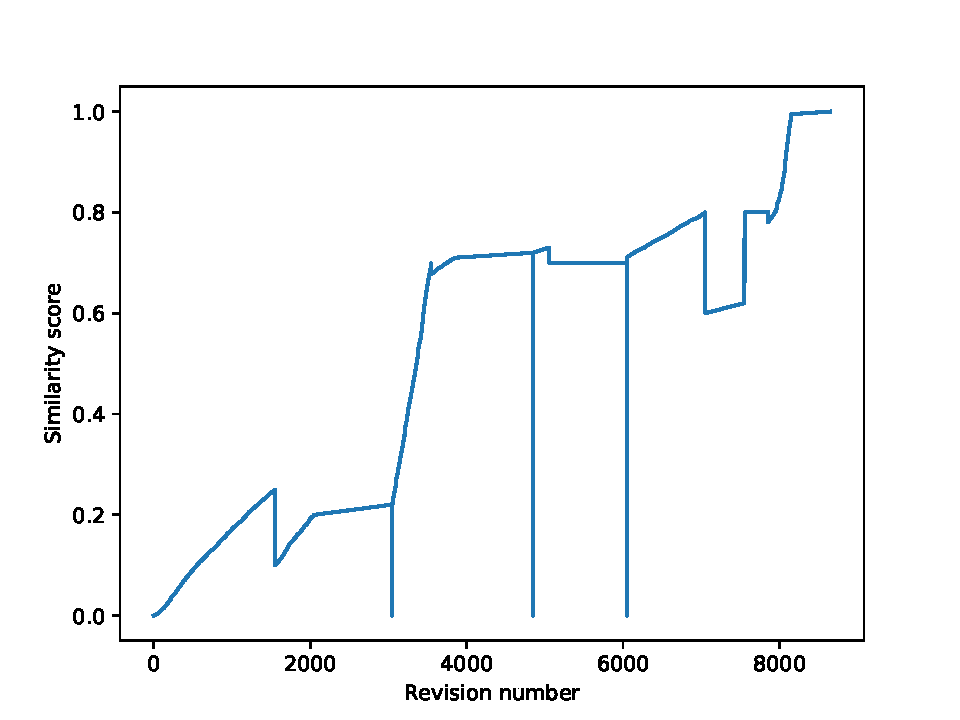
\includegraphics[width= 9cm]{images/similarity_score_stephen2.pdf}
    \caption{\label{fig: similarity_score_stephen2} Plot of similarity score variation with revision.}
\end{figure}

%
%Wikipedia formula:
%\begin{align*}
%Rank(R) = count(distinct(rev\_page))+\\
%sqrt(count(rev\_id)-\\
%count(distinct(rev\_page)))*2 
%\end{align*}

%\subsubsection{Relation between Article Length and it's Reading Extent}


\subsubsection{Relation between Gaze Pattern and Article Readability}

Plot between GL and the time taken to read the text portion.

\begin{figure}[!htb]
    \center 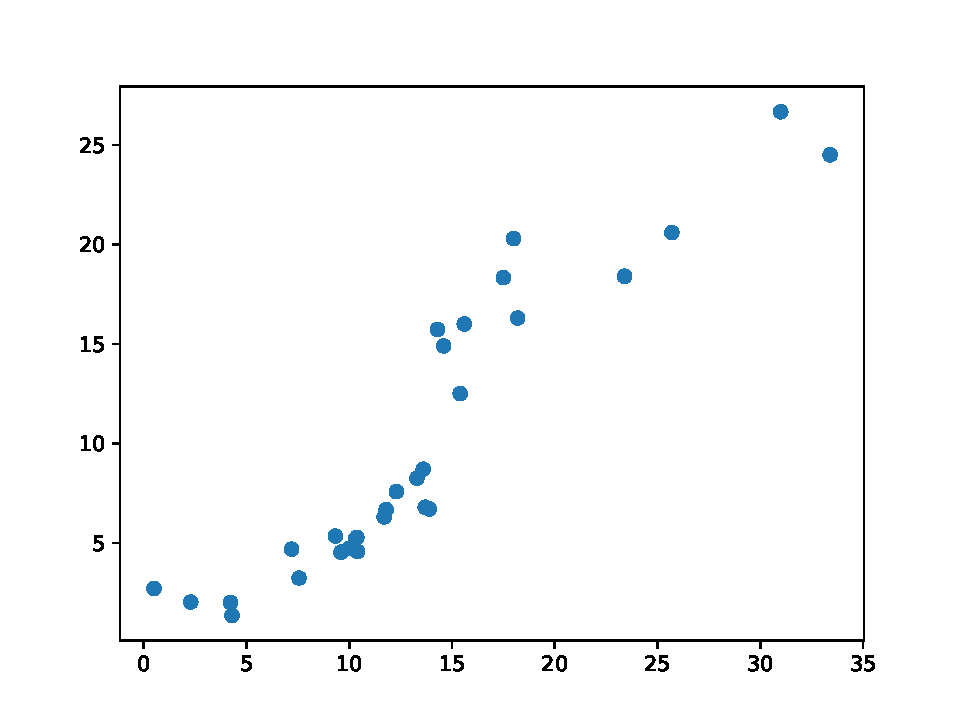
\includegraphics[width= 9cm]{images/GL_time.pdf}
    \caption{\label{fig: GL and time plot} Count articles belonging to various categories}
\end{figure}


    
\section{Online Resources}\label{sec:Resources}


\section{Discussion}\label{sec:Discussion}


\section{Conclusion \& Future Work}\label{sec:Conclusion}

\newpage

\bibliography{neeru} 
\bibliographystyle{ieeetr}

\appendix

\section{Research Methods}

\subsection{Part One}



\subsection{Part Two}


\section{Online Resources}


\section{Words}
``averted" means tiled away

\end{document}
